Famous ancient Greek sculptor Phidias is making preparations to build another marvelous monument. For this purpose he needs rectangular marble plates of sizes $W_1\times H_1, W_2 \times H_2, \ldots, W_N \times H_N$. 

Recently, Phidias has received a large rectangular marble slab. He wants to cut the slab to obtain plates of the desired sizes. Any piece of marble (the slab or the plates cut from it) can be cut either horizontally or vertically into two rectangular plates with integral widths and heights, cutting completely through that piece. This is the only way to cut pieces and pieces cannot be joined together. Since the marble has a pattern on it, the plates cannot be rotated: if Phidias cuts a plate of size A B then it cannot be used as a plate of size B A unless A B. He can make zero or more plates of each desired size. A marble plate is wasted if it is not of any of the desired sizes after all cuts are completed. Phidias wonders how to cut the initial slab so that as little of it as possible will be wasted. 

As an example, assume that in the figure below the width of the original slab is 21 and the height of the original slab is 11, and the desired plate sizes are 10 4, 6 2, 7 5, and 15 10. The minimum possible area wasted is 10, and the figure shows one sequence of cuts with total waste area of size 10. 

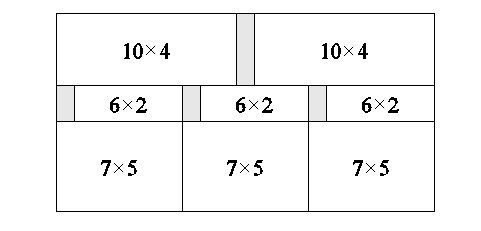
\includegraphics{task2b.jpg}


Your task is to write a program that, given the size of the original slab and the desired plate sizes, calculates the minimum total area of the original slab that must be wasted.
